\section{Aufbau und Durchführung}
\label{sec:Durchführung}

  \subsection{Aufbau}

  Der Versuchsaufbau ist in Abbildung \ref{fig:aufbau} dargestellt.
  Eine Rubidiumspektrallampe emittiert Licht, welches durch eine Sammellinse kollimiert wird.
  Ein Interferenzfilter lässt nur die $D_1$-Linie durch, das Licht wird danach von einem Polarisator zunächst linear polarisiert, um danach durch ein $\lambda/4$-Plättchen rechtszirkular polarisiert zu werden und auf die Dampfzelle zu scheinen. Da das Licht aus einer thermischen Emission stammt, verfügt es über eine Linienbreite, sodass alle im Versuch benötigten Übergänge energetisch erlaubt sind.

  Die Dampfzelle wird beheizt und ist mit einem Gasgemisch aus Rubidium und Neon-Puffergas gefüllt, welches verhindert, dass die Besetzungsinversion durch Stöße des Rubidiums mit den Wänden der Dampfzelle abgeschwächt oder verhindert wird. Stöße zwischen den Rubidium- und Neonatome können keinen Drehimpuls zwischen den Elektronenhüllen austauschen, sodass das Herstellen der Besetzungsinversion dadurch nicht behindert wird. Hinter der Dampfzelle wird das Licht auf eine Photozelle fokussiert, wodurch die Transparenz des Gases für die $D_1$-Linie gemessen wird. Das Signal wird dabei auf den Y-Eingang eines Oszilloskop gegeben.

  \begin{figure}
    \centering
    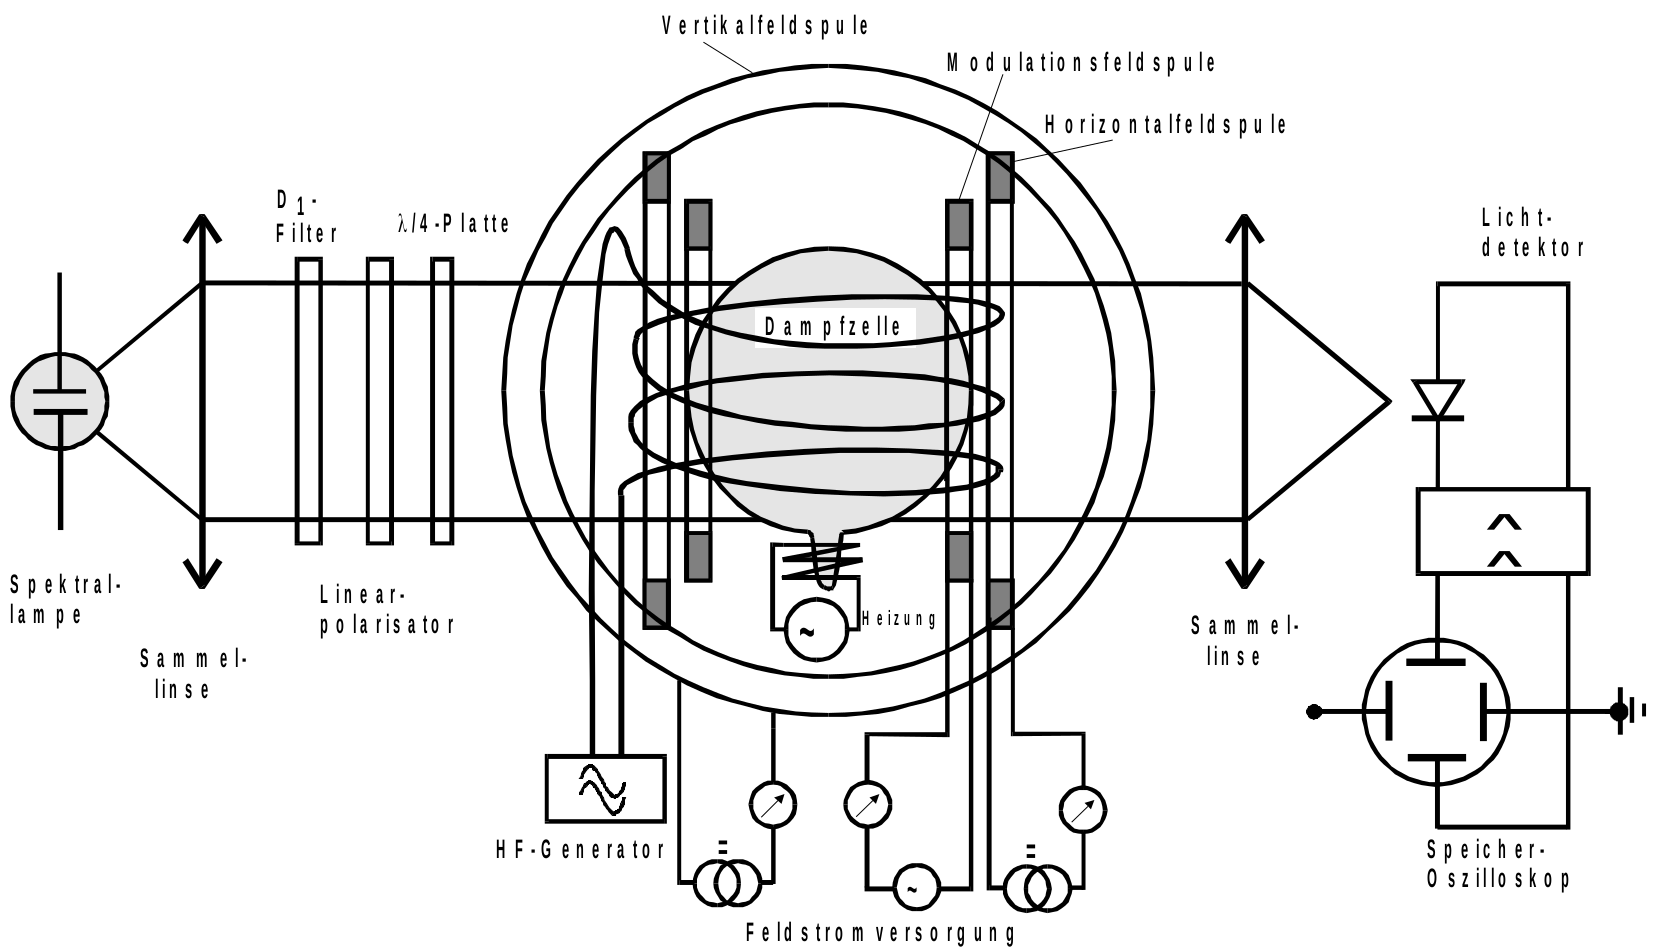
\includegraphics[width=\textwidth]{pictures/aufbau.png}
    \caption{insert description \cite{Versuchsanleitung}.}
    \label{fig:aufbau}
  \end{figure}

  Es stehen drei Helmholtzspulen zur Verfügung, um Magnetfelder anzulegen. Eine Horizontalfeldspule erzeugt ein statisches Horizontalfeld, während die Sweep-Spule auf die Horizontalfeldspule aufgewickelt ist und ein Sägezahnsignal liefert. Das RF-Feld wird mit einem externen Funktionsgenerator angesteuert.

  \subsection{Durchführung}

  Zu Beginn des Versuchs wird der Strahlengang auf eine maximale Intensität eingestellt und die Apparatur abgedeckt, um Streulicht von der Photozelle abzuhalten.
  Das Prinzip der Messung ist, das Sweep-Feld auf den X-Eingang des Oszilloskops zu legen, sodass ein durchlaufender Leuchtpunkt die Intensität in Abhängigkeit der Magnetfeldstärke zeigt.
  Wenn nur das Sweep-Feld angelegt ist, wird ein breiter Dip bzw. Peak zu sehen sein (siehe Nulldip in Abbildung \ref{fig:transparenz}), der dem Erdmagnetfeld zuzuordnen ist. Um seinen Effekt auf die Versuchsdurchführung zu minimieren, wird das Vertikalfeld so eingestellt, dass der Dip möglichst schmal ist und der Tisch in Nord-Süd-Richtung orientiert.

  Um nun die Resonanz bei einer RF-Feldstärke $B_m$ in Abhängigkeit der Frequenz des RF-Feldes zu untersuchen, wird der Frequenzgenerator verwendet. Dieser liefert ein $\SI{4}{\volt}$ Sinus-Signal. Es liegen zwei Dips mit unterschiedlichem $B_m$ vor, da im Gasgemisch zwei verschiedene Rubidium-Isotope vorliegen. Die Messreihe Resonanzfrequenz gegen Magnetfeldstärke wird mithilfe des Sweep-Feldes für Frequenzen zwischen $\SI{100}{\kilo\hertz}$ und $\SI{1}{\mega\hertz}$ aufgenommen.
  Außerdem wird ein Signalbild für eine RF-Frequenz von $\SI{100}{\kilo\hertz}$ aufgenommen, um aus dem Verhältnis der Tiefe der Dips auf das Verhältnis der Isotope im Gasgemisch zu schließen.

  Bei dieser Frequenz wird das Feld resonant eingestellt. Die RF-Spannung wird nun durch eine Rechteckspannung auf dem "Input RF Modulation" mit einer Frequenz von $\SI{5}{\hertz}$ an- und ausgeschaltet. Dieses Signal wird auf Kanal 1 des Oszilloskops gelegt, das in diesem Teil des Versuchs nicht im XY-Betrieb, sondern im YT-Betrieb läuft. Wie in Kapitel \ref{subsec:transient} beschrieben, führt der Spin eine Präzessionsbewegung durch, sodass nach sich eine exponentiell sättigende Transparenz für ein ausgeschaltetes RF-Feld und eine Abschwingung für ein eingeschaltetes RF-Feld ergibt. Die Periodendauer dieser Oszillationen wird für Amplituden von 2 bis $\SI{10}{\volt}$ für beide Isotope, also unterschiedliche Resonanzmagnetfeldstärken, bestimmt.
  Des Weiteren werden Bilder der sättigenden Exponentialfunktionen angefertigt.
